\documentclass[noindent]{tudreport}
\usepackage[utf8]{inputenc}
\usepackage[german]{babel}
\usepackage{amsmath}
\usepackage{listings}
\title{TUDas - Organisationsapp der Technischen Universität Darmstadt}
\subtitle{Ergebnis des E-Learning Projektpraktikums WS18-19}
\subsubtitle{Benedikt Lins (1799381) und Stefan Thaut (1800351)\\
			Fachbereich 20 - Informatik\\
			\today}
\setlength{\parindent}{0em} 

\DeclareMathOperator{\start}{start}
\DeclareMathOperator{\getEnd}{end}
\DeclareMathOperator{\hour}{hour}

\begin{document}
	\lstset{language=Java}
	\maketitle
	\tableofcontents
	
	\chapter{Motivation}
		Jeder Student oder der, der einmal einer gewesen ist, kennt es: Du kommst das erste Mal in die Uni und hast keine Ahnung, was zu tun ist. Alles ist komplett neu und Du bist froh, wenn Du die Räume findest, in denen Du Dich laut Deinem Willkommensbrief einfinden sollst. Selbst wenn Du dann nach ein paar Tagen herausgefunden hast, welche Straßenbahn Dich in die Uni bringt, bist Du nach ein paar Wochen immer noch ratlos, welche Dokumente du gegebenenfalls wo nachreichen musst, wo Du Dich zu welchen Veranstaltungen und Prüfungen anmelden sollst und in welchem Kellerraum nun dieser Treffpunkt Mathe stattfindet.\\
		
		Diesem Problem soll sich die (Android-)App \textit{TUDas} widmen. Die App soll als Organisationsplattform für Studenten verschiedener Fachbereiche während ihres ersten Semesters dienen. Dabei soll TUDas vorhandene Plattformen, wie \textit{Moodle}\footnote{www.moodle.tu-darmstadt.de [zuletzt aufgerufen: 23.11.2018]} oder die \textit{OAPP} \footnote{www.oapp.tu-darmstadt.de [zuletzt aufgerufen: 23.11.2018]} unterstützen und nicht ersetzen.\\
		%TODO worin unterscheidet sich die App von OAPP und Moodle und Google Maps etc?
		
		Diese Dokumentation soll einerseits die Funktionalitäten der App TUDas festhalten und andererseits als Übersicht für zukünftige Entwickler dienen. Kapitel \ref{chap:technical_specifications} behandelt die technischen Spezifikationen der App. In Kapitel \ref{chap:functionalities} werden die Features beschrieben, die von der App in ihrer jeweils aktuellen Version angeboten werden. Und Kapitel \ref{chap:documentation} beinhaltet eine Dokumentation des Codes.
		
	\chapter{Technische Spezifikationen}\label{chap:technical_specifications}
		Aus Zeit- und Komplexitätsgründen wird die App zunächst nur für das \textit{Android}-Betriebssystem\footnote{https://www.android.com/ [zuletzt aufgerufen: 24.11.2018]} entwickelt.
	
	\chapter{Funktionalitäten}\label{chap:functionalities}
		Dieses Kapitel beschreibt die Funktionalitäten, die die App in ihrer jeweils aktuellen Version anbietet. Dabei sollen die jeweiligen funktionalen sowie nicht-funktionalen Anforderungen aufgezeigt werden und nicht die programmiertechnische Umsetzung, die dann in Kapitel \ref{chap:documentation} folgt.
		
		\section{Campus-Navigation}\label{sec:campus_navigation}
		
		\section{Stundenplan}\label{sec:timetable}
			Im Stundenplan sollen die Termine des Nutzers angezeigt werden. Dies sind sowohl die selbst erstellten Einträge des Nutzers als auch die Termine von abbonierten Veranstaltungen. Üblicherweise beinhaltet ein Stundenplan Einträge, die sich wöchentlich wiederholen. Fristen oder Termine in abbonierten Listen haben einen überwiegend einmaligen Charakter. Daher können hier zwei grundsätzliche Typen von Terminen unterschieden werden:
			\begin{itemize}
				\item Einfache Termine
				
				\item Wiederholende Termine
			\end{itemize}
			Die Charakteristik der wiederholenden Termine impliziert eine einmalige Anzeige im Stundenplan an einem bestimmten Datum. Daher ist es sinnvoll, den Stundenplan datumsabhängig anzuzeigen. Da die Bildschirmbreite des Smartphones in der vertikalen Ausrichtung deutlich begrenzt ist, muss auch die Anzahl der angezeigten Tage beschränkt werden. Zwei Tage, das heißt also der aktuelle Tag und der darauffolgende Tag, scheint eine sinnvolle Wahl zu sein, da man an diesen Tagen gegenwärtig am meisten interessiert ist. Der entsprechende Wochentag mit dem dazugehörigen Datum wird in einer Kopfzeile angezeigt. Auf der linken Seite sind in vertikaler Ausrichtung die Uhrzeiten in stündlichem Abstand untereinander angeordnet. Dabei beginnt der Stundenplan oben mit der maximalen ganzen Stunde, die kleiner als oder gleich allen Anfangsuhrzeiten von Terminen im angezeigten Zeitraum ist und endet unten mit der minimalen ganzen Stunde, die größer als oder gleich allen Enduhrzeiten der gleichen Termine sind.
		
		\section{Variabel einsetzbare, moderierbare Aufgabenlisten}\label{sec:todo_list}
		
	\chapter{Dokumentation der Implementierung}\label{chap:documentation}
		\section{Stundenplan}
			Wie in Abschnitt \ref{sec:timetable} beschrieben, müssen grundlegend zwei Arten von Terminen unterschieden werden. Ein wiederholender Termin hat im Vergleich zu einem einfachen Termin zusätzlich ein Startdatum, an dem die Wiederholung des Termins beginnt und ein Enddatum, wann die Wiederholung endet. Notwendig ist ebenfalls eine Wiederholungsvorschrift. Möchte man nun eine Teilmenge von wiederholenden Terminen löschen, so ist es notwendig, dass die Termine nicht zur Laufzeit auf Grundlage der Wiederholungsvorschrift berechnet werden sondern die Termine schon gespeichert wurden. Ansonsten wäre es nicht möglich zu spezifizieren, welche Termine von der Wiederholungsvorschrift ausgeschlossen werden sollen. Die wiederholenden Termine unterscheiden sich dann nur noch in den Daten. Der Titel und die Beschreibung beispielsweise sind für alle wiederholenden Termine jeweils gleich. Um Redundanzen zu vermeiden, werden solche Attribute von den reinen Datumsangaben getrennt. Die Klasse \lstinline!AppointmentContent! beinhaltet die statischen Informationen einer Terminsammlung und die Klasse \lstinline!Appointment! enthält die Datumsangaben. Die Attribute der Klassen sind im UML-Diagramm in Abbildung \ref{fig:uml_appointment} zu sehen.\\
			Für eine mathematische Beschreibung des Projekts müssen diverse Hilfsfunktionen definiert werden. Sei $A$ die Menge aller Termine des Benutzers und $\mathbb{D}$ die Menge aller Datumsangaben, die auch den Zeitpunkt am Tag beinhalten. Die Funktion
			\begin{align}
\start: A \rightarrow \mathbb{D} \label{fun:start}
			\end{align}
			liefert für einen gegebenen Termin den Startzeitpunkt. Analog liefert die Funktion
			\begin{align}
\getEnd: A \rightarrow \mathbb{D} \label{fun:end}
			\end{align}
			den Endzeitpunkt des gegebenen Termins. Für eine bestimmte Datumsangabe gibt die Funktion
			\begin{align}
\hour: \mathbb{D} \rightarrow \{0, \dots, 23\} \label{fun:hour}
			\end{align}
			die Stunde der Angabe aus.
			
			\begin{figure}[h]
				\centering
				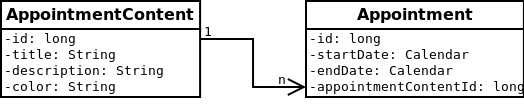
\includegraphics[scale=0.5]{img/uml_appointment.png}
				\caption{UML-Diagramm der Klassen \lstinline!AppointmentContent! und \lstinline!Appointment!}
				\label{fig:uml_appointment}
			\end{figure}
			
			\subsection{Modellierung der Anfangs- und Endzeitbedingung}
				Die in Abschnitt \ref{sec:timetable} beschriebene Anforderung, dass der Stundenplan mit der maximalen Stunde beginnen soll, die kleiner als die Startzeiten aller Termine im betrachteten Zeitraum ist, kann wie folgt formalisiert werden: Für ein gegebenes Start- und Enddatum $s \in \mathbb{D}$, bzw. $e \in \mathbb{D}$ ist
				\begin{align}
A_f = \{a \in A: s \leq a \leq e\}
				\end{align}
				die Menge aller Termine im gegebenen Zeitraum. Dann ist die gesuchte Stunde $h$, zu der der Stundenplan beginnen soll, mithilfe der Funktionen \ref{fun:start} und \ref{fun:hour} wie folgt definiert:
				\begin{align}
h_s = \max\{h_s \in \{0, \dots, 23\}: \forall a \in A_f: h_s \leq \hour(\start(a)) \}
				\end{align}
				Analog ist die Stunde der Endzeit $h_e$ definiert:
				\begin{align}
h_e = \min\{h_e \in \{0, \dots, 23\}: \forall a \in A_f: h_e \geq \hour(\getEnd(a)) \}
				\end{align}

\end{document}